\chapter{Csend}

\section{Jelzés}

\keywords{kapcsolat a környezetünkkel}

\noindent Ketten sétálunk a kolostor bejáratához vezető úton.
Beszélgetünk erről és arról, de amikor belépünk, észrevesszük a csendet
és a párbeszédünk abbamarad. A Dhamma terem a következő ajtón túl van,
és nem akarunk zavarni senkit, aki esetleg odabent meditál. Halkan
bezárjuk magunk mögött az ajtót. Mi az épület egy másik részébe tartunk,
de a Dhamma terem jelentősége nagyobb ennél a hétköznapi feladatnál.

A hallgatás csendje egy implicit kapcsolatot teremt a környezetünkkel.
Az előbbi esetben azzal a személlyel, aki lehet, hogy a Dhamma teremben
ül. Még ha látnánk is, hogy nincs ott senki, akkor is lehalkítanánk a
beszédünket vagy csendben maradnánk. Amikor belépünk, a csend jelzésként
szolgál arra, hogy figyeljünk. Teret adunk az önmagunkon túli
értékeknek, melyeket az szív és elme igazságainak szentelt Dhamma terem
jelképez.

Ebben a környezetben a csend jelzés, ami arra irányít, hogy emlékezzünk
arra, amit a világi értékeken túl van. Amikor egy templomba, kolostorba
vagy más megszentelt helyre lépünk be, a zajos világi ügyeken túlra
tekintünk, túl az önmagunkra irányuló megszokott elfoglaltságunkon.

Elég tapasztalatunk van a zajos csacsogásban ahhoz, hogy tudjuk, a mély
megértés nem abban található. Ezért elcsendesülünk, hogy figyelmünket a
hallgatásnak adhassuk, hogy része legyünk a megértésnek, amit szavakkal
nem tudunk kifejezni. Csendben mozgunk, csendben hallgatunk. Óvatosan
eltávolítjuk magunkat az útból, hogy meghallhassuk a hely üzenetét és
engedjük a cselekvést magáért beszélni. A csend jelenlétet ad, ami nem
elkülönít, hanem magába foglalja a teret és az ott élő más lényeket.
David Whyte szavaival,\footnote{\href{https://www.goodreads.com/quotes/10119971-the-winter-of-listening-no-one-but-me-by-the}{The
  Winter of Listening by David Whyte}}

\begin{quote}
Tartozhatsz mindenhez:\\
csak hallgass csendben.
\end{quote}

\section{Értékes}

\keywords{a csend értéke, nyugalom a csendben}

\noindent A csend azt is kifejezi, mennyire értékeljük amit éppen
teszünk. Csendben lenni és fenntartani a figyelmünket kifejezi az
éberséget és tiszteletet a cselevés iránt. Ez egyaránt egy belső és
külső jelzés: Mások látják, hogy bármi is legyen amit csinálunk, csendre
van szükségünk. Mi is látjuk önmagunkat ahogy csendben vagyunk, mikor
szándékosan visszafogjuk hatásunkat magunkra és a környezetünkre. Ezzel
kommunikáljuk, hogy ahol vagyunk és amit teszünk nagyobb jelentőséggel
bír, mint magunkról csacsogni.

A nyugalom, megértés és csend közeli kapcsolatban állnak egymással.
Felhagyunk a beszéddel és óvatosan figyelünk, hogy vizsgálódjunk és
megértsünk egy jelenséget. A verbális csendet követően, az elme
folytatja, `Miért? Miért?' De amikor összeáll a kép az `Aha!'
pillanatában, az elme megáll a belső párbeszédben és csendben vagyunk,
örömmel tölt el minket a megértés. Ebben az elégedett, nyugodt
hangulatban csendben maradunk. Pillanatnyilag semmi másra nincs
szükségünk.

\begin{quote}
Mint egy tiszta vizű,\\
nyugodt és mély tó, olyan\\
a bölcs, aki miután hallott\\
a dharmákról, lecsendesült.

\bigskip

\quoteRef{%

Dhammapada 82, ford. Fórizs László

}
\end{quote}

\section{Fekvő meditáció módszere}

\noindent A testi nyugalom a fekvő meditáció módszerére a legjellemzőbb.
Ebben a testhelyzetben az izmok teljesen ellazulnak. Habár ez megteremti
a könnyedség és kényelem érzetét, oda kell figyelnünk, hogy elkerüljük
az elalvást. Amikor testileg el vagy fáradva, ez a testtartás nem
javasolt formális meditációra. Ehelyett az ülő, sétáló vagy álló
meditáció megfelelőbb, mivel ezek növelik a test éberségének szintjét az
erőfeszítésen keresztül.

\clearpage
\thispagestyle{empty}\mbox{}
\contentFullBleed{%
\centering
\null\vfill

\hspace*{20mm}%
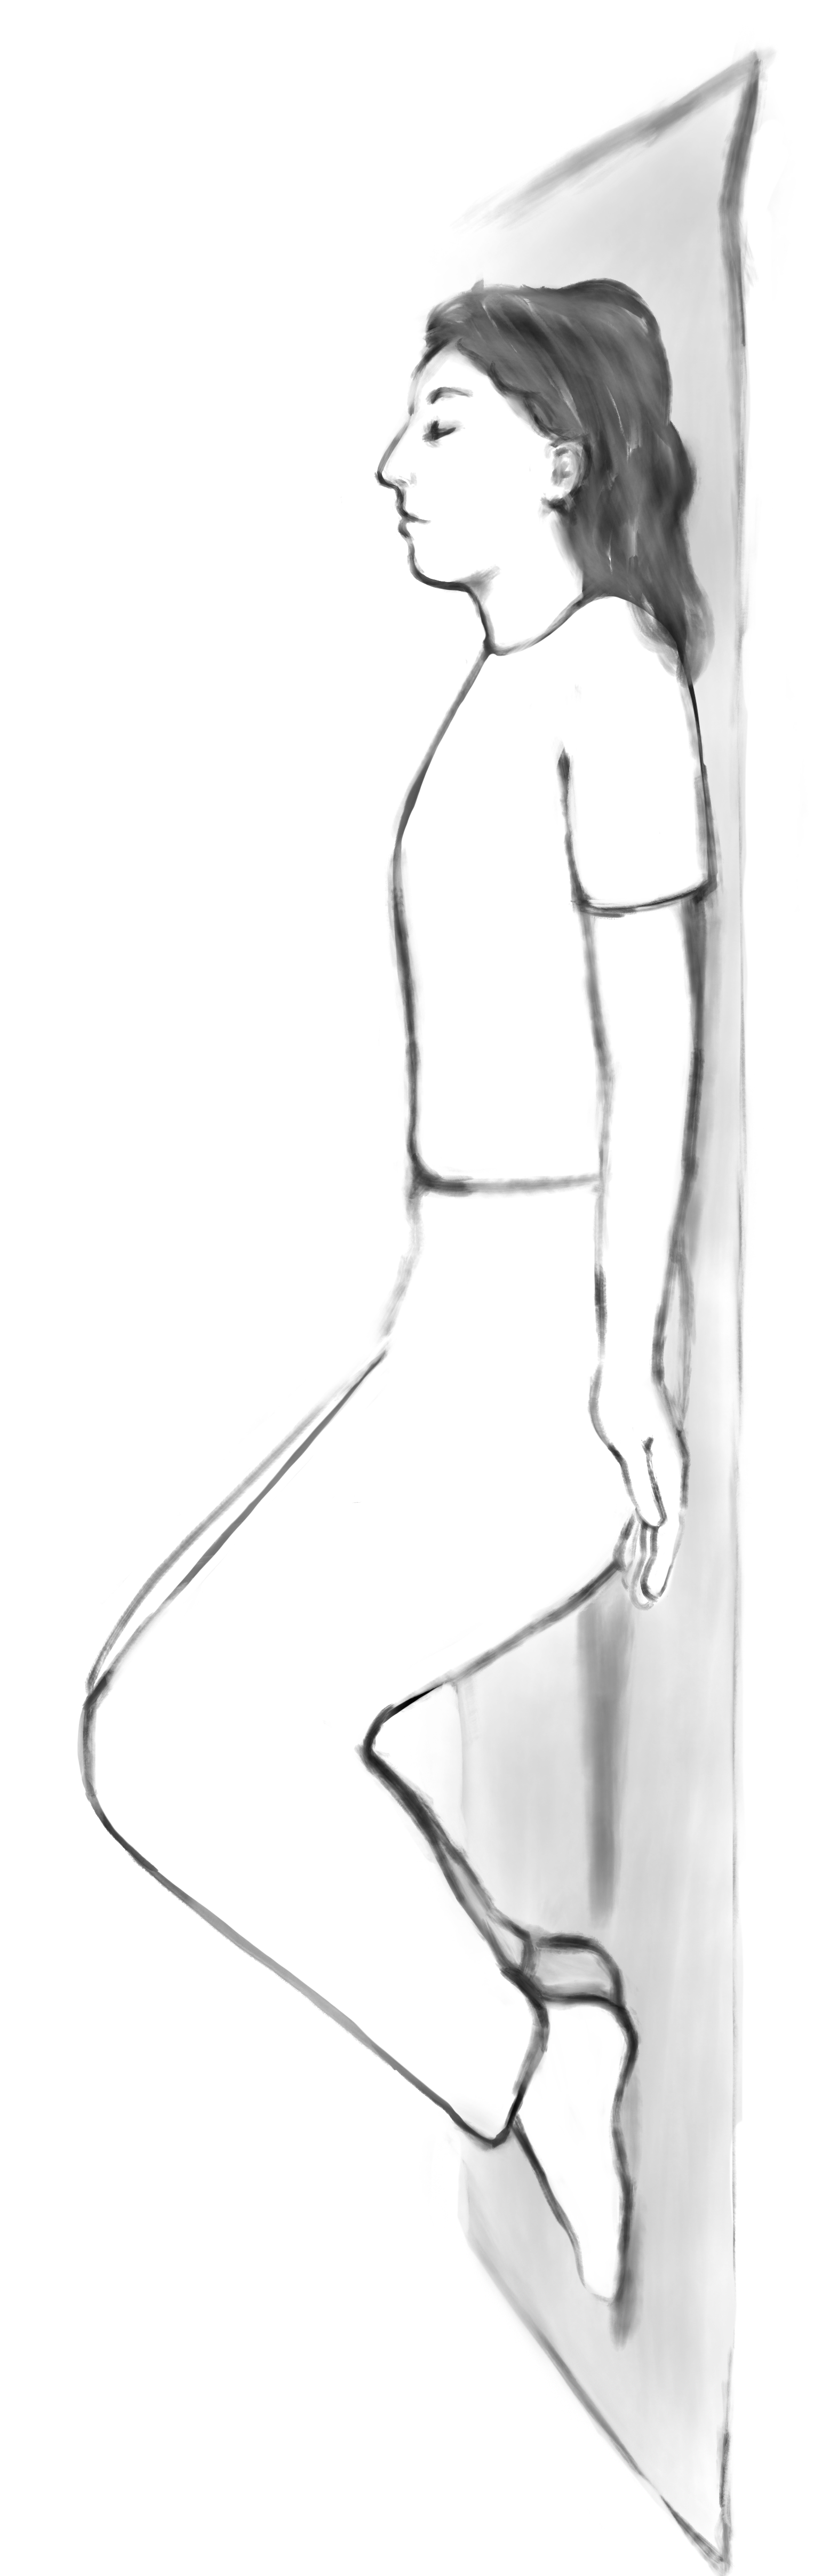
\includegraphics[height=190mm]{lying-down.png}

\illustration{Fekvő Meditáció Testtartás}%
\label{illus-lying-down-meditation}%

\vfill\null
}
\clearpage

Mielőtt lefeküdnél, határozd meg tisztán a szándékot, hogy éber leszel.
Ez megfelelő hozzáállást teremt, és némi mentális távolságot hoz létre a
napközbeni feladatainktól. Tovább fejleszthetjük a tiszteletteljes
hozzáállást azzal, hogy leborulást végzünk egy Buddha szobor irányába,
és halkan recitálunk egy rövid kántálást.

Egy jóga matrac, vagy puha szőnyeg hasznos, hogy elkerüljük a kemény
padló miatt fájó testrészeket. Ha úgy érzed, hogy a légzésed
akadályozott, miközben a fej hátra hajlik, használj egy kis méretű
párnát, vagy összehajtott törülközőt arra, hogy megtartsa a fejet. Az
ágyban feküdni lehet, hogy túl puha lesz, és a testet az alvásra
emlékezteti.

Engedd a karokat a test mellett pihenni; ha a hasra vagy a mellkasra
helyezed őket, az emelkedő és süllyedő mozgás könnyen elvonja a
figyelmed. Húzd fel a térdeket, hogy a talpak egyenletesen feküdjenek a
szőnyegen és az alsó hátat közelebb engedje a padlóhoz. Ez elkerüli az
ízületekben a feszültséget és segít fenntartani az éberséget.

Tartsd meg ezt a tartást, miközben ellazítod az test izmait és a testi
nyugalmat fejleszted. Irányítsd a figyelmet befelé, használd a légzés
érzetét mint meditációs tárgyat. Kísérletezz a légzéssel. Használd arra,
hogy felélénkítsd az elmét és megőrizd a tiszta éberséget. Ha az elme
elsodródik a szürke tompaság felé, ezt álmosság fogja követni. Egy órát,
vagy időzítő jelzést beállítani hasznos lehet, vagy a meditáció végét
jelezni, vagy mint egy időszakos emlékeztető arra, hogy éber maradj.

\clearpage

\section{A hangok hatása}

\keywords{zajnak kitéve lenni, szabad kognitív kapacitás}

\noindent Ez nem jelenti, hogy a hang nem lehet kellemes. A zene
terápiás hatásai nyilvánvalóak, és segít ellazítani a feszült elmét.
Lehet, hogy \emph{nagyon jó a zene} (a mi véleményünk szerint), de
hányszor tudod meghallgatni egymás után? Ugyanaz a dolog újra és újra,
rövid idő alatt kellemesből fájdalmasba fordul át. Voltál már úgy, hogy
órákig zenét hallgattál, de mégis megkönnyebbülve érezted magad, mikor
kikapcsoltad? `Jó zene, de már hiányzott a csend.'

A hangok bejövő jelek, amik stimulálják az idegrendszert. Egyes hangok
jó érzést kelthetnek egy ideig, pozitív hatással, míg más hangok
irritációt és szétszórtságot okoznak.

A zajos környezet rontja a figyelmünk és intelligenciánk minőségét.
Valószínűleg emlékszel arra, milyen nehéz tisztán gondolkodni amikor a
szomszéd telkén építkezési munkák folynak. A személyes tapasztalaton
túl, orvosi tanulmányok is felmérték, hogy `a szellemi munkavégzés és
látási / hallási figyelem jelentősen csökken'\footnote{\href{https://www.ncbi.nlm.nih.gov/pmc/articles/PMC6901841/}{The
  Effect of Noise Exposure on Cognitive Performance and Brain Activity
  Patterns (ncbi.nlm.nih.gov)}} mikor zajnak vagyunk kitéve.

A mobiltelefonoknak még hangot sem kell kiadniuk, hogy `leszívják az
agyat': egy másik tanulmány azt találta, hogy `a saját telefonunk puszta
jelenléte csökkenti az elérhető szellemi kapacitást'.\footnote{\href{https://www.journals.uchicago.edu/doi/10.1086/691462}{Brain
  Drain: The Mere Presence of One's Own Smartphone Reduces Available
  Cognitive Capacity (journals.uchicago.edu)}}

Nem meglepő, hogy a hagyományos belátás meditációt tanító elvonulások
igyekeznek csendes környezetet teremteni, és arra kérik a résztvevőket,
hogy ne hozzák be a telefonjukat a meditációs terembe, vagy hagyják azt
egy elzárt helyen az egész elvonulás idejére. Adj egy kis szünetet az
idegrendszernek és engedd lecsillapodni. Ne járjon úgy mint a varjú
Szantóka haiku versében,\footnote{\href{https://www.goodreads.com/book/show/931086.Grass_and_Tree_Cairn}{Grass
  and Tree Cairn, Taneda Santoka}}

\begin{quote}
Károg a varjú,\\
csapkod a varjú,\\
nincs ahol megüljön.
\end{quote}

\section{Kántálás}

\keywords{tiszán meghatározni a szándékot, jótékony gondolatok}

\noindent A kolostorban kántálást gyakorlunk a mindennapos közös
meditációk előtt vagy után. Először, amikor egyenként megérkezünk a
Dhamma terembe, csendben három leborulást végzünk a Buddha oltár
irányába. A rangidős szerzetes megcsengeti a harangot, ezzel jelzi a
kántálás kezdetét. Csendben várunk, miközben meggyújtja az oltáron a
gyertyákat és füstölő pálcákat, majd újra meghajlunk. A leborulás közben
mindig csend van.

Együtt elkezdjük a kántálást, összehangolva a hangunkat: a halkat nem
lehet hallani, a hangos túl erős, a hamis kiválik az összhang
harmóniájából. (Egy jó irányelv, ha nem hallod a saját hangod, akkor túl
halkan kántálsz. Ha csak a saját hangodat hallod, túl hangos vagy.)

A kántálások szövegei a Buddhát és a tanításokat idézik fel, ez a
gyakorlat az elmét jótékony gondolatok irányába vezérli. Az ilyen
rendezett, szimbolikus ceremónia a beszéd és test ritmusát használja,
mint alkalmas eszközt arra, hogy kitisztítsa az elmét a meditáció
csendje előtt.

A pontos rutin kolostoronként változik. A Szumédháráma kolostorban
Portugáliában a reggeli mediáció 5 órakor kezdődik. Egy óra ülő
meditációval kezdünk, ami alatt nincs beszéd vagy kántálás. Amikor
belépsz, csend van -- a belső vizsgálódásra szánt megosztott tér. A
meditáció végén a rangidős szerzetes megcsengeti a harangot, amit 15-20
perc kántálás követ.

\section{Unalom}

\keywords{unalom, az eméről tanulni, belső béke, érzéki visszafogottság}

\noindent `Nem unalmas egy idő után?' Időnként egy-egy iskolai program
egy egész osztály gyereket elhoz a kolostorba, hogy csendben
meditáljanak (talán azt remélve, hogy később csendesebbek lesznek). Ők
valószínűleg szörnyen unják magukat. Kezdettől fogva nem érdekelte őket,
hogy ott legyenek, de a gyerekek okosak, és gyakran megtanulják, hogy
hamarabb szabadulnak, ha elviselik a felnőttek furcsa ötleteit.

Amikor a rendszeres látogatóink jönnek meditálni, kezdettől fogva más a
hozzáállásuk ehhez az elmeállapothoz. Úgy érkeznek, hogy érdekli őket,
hogy magukról és az elméjükről tanuljanak. Amikor közelebbről megnézed
azt, ami `unalmas', hamar érdekessé tud válni. Az unalom megváltozik
amint ránézel. `Nem sok minden történik, csak a lélegzés. Probléma ez
nekem? Én hozom létre azt a problémát? Meg tudom állítani, hogy ilyen
problémákat gyártsak magamnak? Itt ülni és lélegezni tulajdonképpen
kellemes érzés.'

Miközben a légzésre való éberséget gyakoroljuk, megjelenik az öröm, ami
az érzékek visszafogottságából születik. Az elme ellazul, és a
gondolkodást engedhetjük megállni. Csendben vizsgáljuk a
tapasztalatunkat, nincs szükség azt kommentálni.

Az unalom a tényezők egy kombinációja: a vágy az izgalomra és
újdonságra, a jelen aktív elutasítása, és a hozzáállás, hogy már tudjuk
mi fog történni. Nem a helyzet magából eredő tulajdonsága, hanem a
képzetlen, nyugtalan elme szokása.

A Buddha a nyugtalanságot ahhoz hasonlította, mint ahogy egy elefánt
érzi magát, amikor az állatidomár első ízben megfékezi azzal, hogy
kiköti egy erős oszlophoz. Az elefánt alkalmatlan a kiképzésre, amíg
folyton arra vágyik, hogy a vadonban kóboroljon amerre csak akar. Egy jó
idomár fokozatosan megfékezi a nyugtalan elefántot, amíg az meg nem
tanul nyugton maradni.\footnote{\href{https://suttacentral.net/mn125}{MN
  125}, The Level of the Tamed} A szuttában, Dzsajaszéna herceg, aki a
palotában él, ahol a figyelemelterelő szórakoztatás veszi őt körbe, el
sem hiszi, hogy a belső békét lehetséges elérni az érzékek visszafogásán
keresztül, hiszen maga sosem tapasztalt még ilyen békét.

A meditációs terem ajtaja mindig nyitva van, bármikor felállhatsz és
kisétálhatsz. De azért vagy ott, mert érezted, hogy a képzetlen elme
állandóan fájdalmas hibákba és gondokba kevert. Ha ezer lépést teszel
ezer irányba, csak elfáradsz, és mérgelődhetsz, hogy miért nem jutottál
sehova. Helyes dolog felismerni a szükséget, hogy saját nyugtalan elménk
idomárai legyünk. Megtanuljuk mi a helyes irány, és arra felé teszünk
lépéseket.

\begin{quote}
A nehezen megfékezhető,\\
csapongó, vágyűzött elme\\
ellenőrzése jó. A megfékezett\\
elme boldogságot hordoz.

\bigskip

\quoteRef{%

Dhammapada 35, ford. Fórizs László

}
\end{quote}

\section{Oltár}

\keywords{szent helyeket létrhozni, egy Buddha oltár szimbólumai}

\noindent Nem mindig készítettem Buddha oltárat a szobában vagy
kunyhóban ahol éppen szállásom volt a kolostorban. Kezdetben azt
gondoltam, hogy az intézményes elvárásokhoz való igazodásban volt
szerepük. Így többnyire figyelmen kívül hagytam őket, és némileg
nehezteltem a képekre és szobrokra. Úgy éreztem mások azt várják el
tőlem, hogy tiszteljem azokat, és ellentartó hozzáállással nem akartam
azt tenni, amit (úgy gondoltam) elvárnak tőlem.

A reakcióm olyan volt, mint az iskolás gyerekeké: elég okos voltam
ahhoz, hogy elviseljem a szimbólumokat, és elég arrogáns ahhoz, hogy azt
higgyem én már tudom mit jelentenek. Aki okosnak gondolja magát,
felületesen elutasít mindent, és unalmassá válik számára a világ. Ez egy
önbutító kombináció. Azt gondolni, hogy \emph{én már tudom}, bezárja az
elmét, így nem tudsz rájönni, hogy valójában nem tudod. A brit
pszichológus Iain McGilchrist ahhoz hasonlítja ezt, mintha beragadtunk
volna egy tükrökből álló labirintusba:\footnote{\href{https://www.goodreads.com/book/show/6968772-the-master-and-his-emissary}{The
  Master and His Emissary: The Divided Brain and the Making of the
  Western World by Iain McGilchrist}} csak azt látod, amit te mondasz
magadnak, és sosem találod meg a kiutat.

Egy kis repedés jelenhetett meg azokon a tükrökön, mert észrevettem,
hogy tulajdonképpen senki nem gondolt rám ilyen ítélettel és elvárással.
Én magam hoztam létre a történet mindkét oldalát, és olyasmi miatt
emésztettem magam amit csak képzeltem.

Egy Buddha oltárt készíteni egy kis teret hoz létre a helyen ahol élünk,
egy emlékeztető arra, hogy álljunk meg a rohanásban és adjunk teret a
felébredésnek. A meditációs terem ugyanezt az üzenetet adja át nekünk a
csenden keresztül. Egy oltár ajándék nekünk, magunktól. Nem azért van,
hogy mások elvárásainak feleljen, vagy akár a Buddhának. A történelmi
Buddha 2600 évvel ezelőtt elhunyt, és túl van azon, hogy tőlünk bármire
is szüksége legyen. Másoknak van elég dolguk amin aggódhatnak, és nem
gondolnak annyit ránk mint azt képzeljük.

Emlékszem arra gondoltam, `Miért nincs helyem a Buddha számára ott, ahol
élek?' Neki is láttam levágni néhány fadeszkát és készítettem egy kis
polcot az oltárnak. A Buddha oltárak gyakran elég egyszerűek: egy vagy
több Buddha szobor, gyertyák, füstölő és virágok. A Buddha jelképezi a
felébredett tudatosságot az emberi formában. A gyertyák a bölcsességnek
felelnek meg, ami láthatóvá teszi a dolgokat, mint a fény a sötétségben.
A füstölő eszünkbe juttathatja, amikor a Buddha a jóságról beszélt: `Se
szantálfa, se tagara, se jázmin illata nem száll a szél ellenében, a
jóság viszont szembeszáll a széllel, a jó áthatja az egész
világot.'\footnote{Dhammapada 54, ford. Fórizs László} A virágok az
erényes tettek, boldogság és állandótlanság szimbólumai. Olyanok, mint a
gyakorlásunk: boldogságot hoznak, ha jól gondoskodunk róluk;
elhervadásuk pedig emlékeztet minket az állandótlanságra.

Felajánlom ezeket a vizsgálódó szavakat azzal a szándékkal, hogy
bátorítsanak a gyakorlásban. A tanító a Buddha, a megvilágosító
magyarázatok forrása hozzá vezet vissza. Hálás vagyok azért, hogy a
tanításait egyik generáció a másik után továbbhordozta a sok évszázadon
át a mai napig. Használjuk fel arra, hogy az elme zajos kavargását
átalakítsuk megértő csenddé.
